\documentclass[conference]{IEEEtran}

\usepackage{graphicx}
\usepackage{xcolor}
\usepackage[hidelinks]{hyperref}

\graphicspath{{figures/icnp_graphs/}}

\title{QuantumFaultTolerant ICNP Result Plot Pack}
\author{Piter Garcia}

\begin{document}
\maketitle

\begin{abstract}
This standalone plot pack collects the seven ICNP candidate result figures generated from the validated result artifacts. It is a review artifact; the G7 synthesis panel is also included in \texttt{main.tex} as the current synthesis figure.
\end{abstract}

\section{Candidate Result Figures}

\begin{figure*}[t]
    \centering
    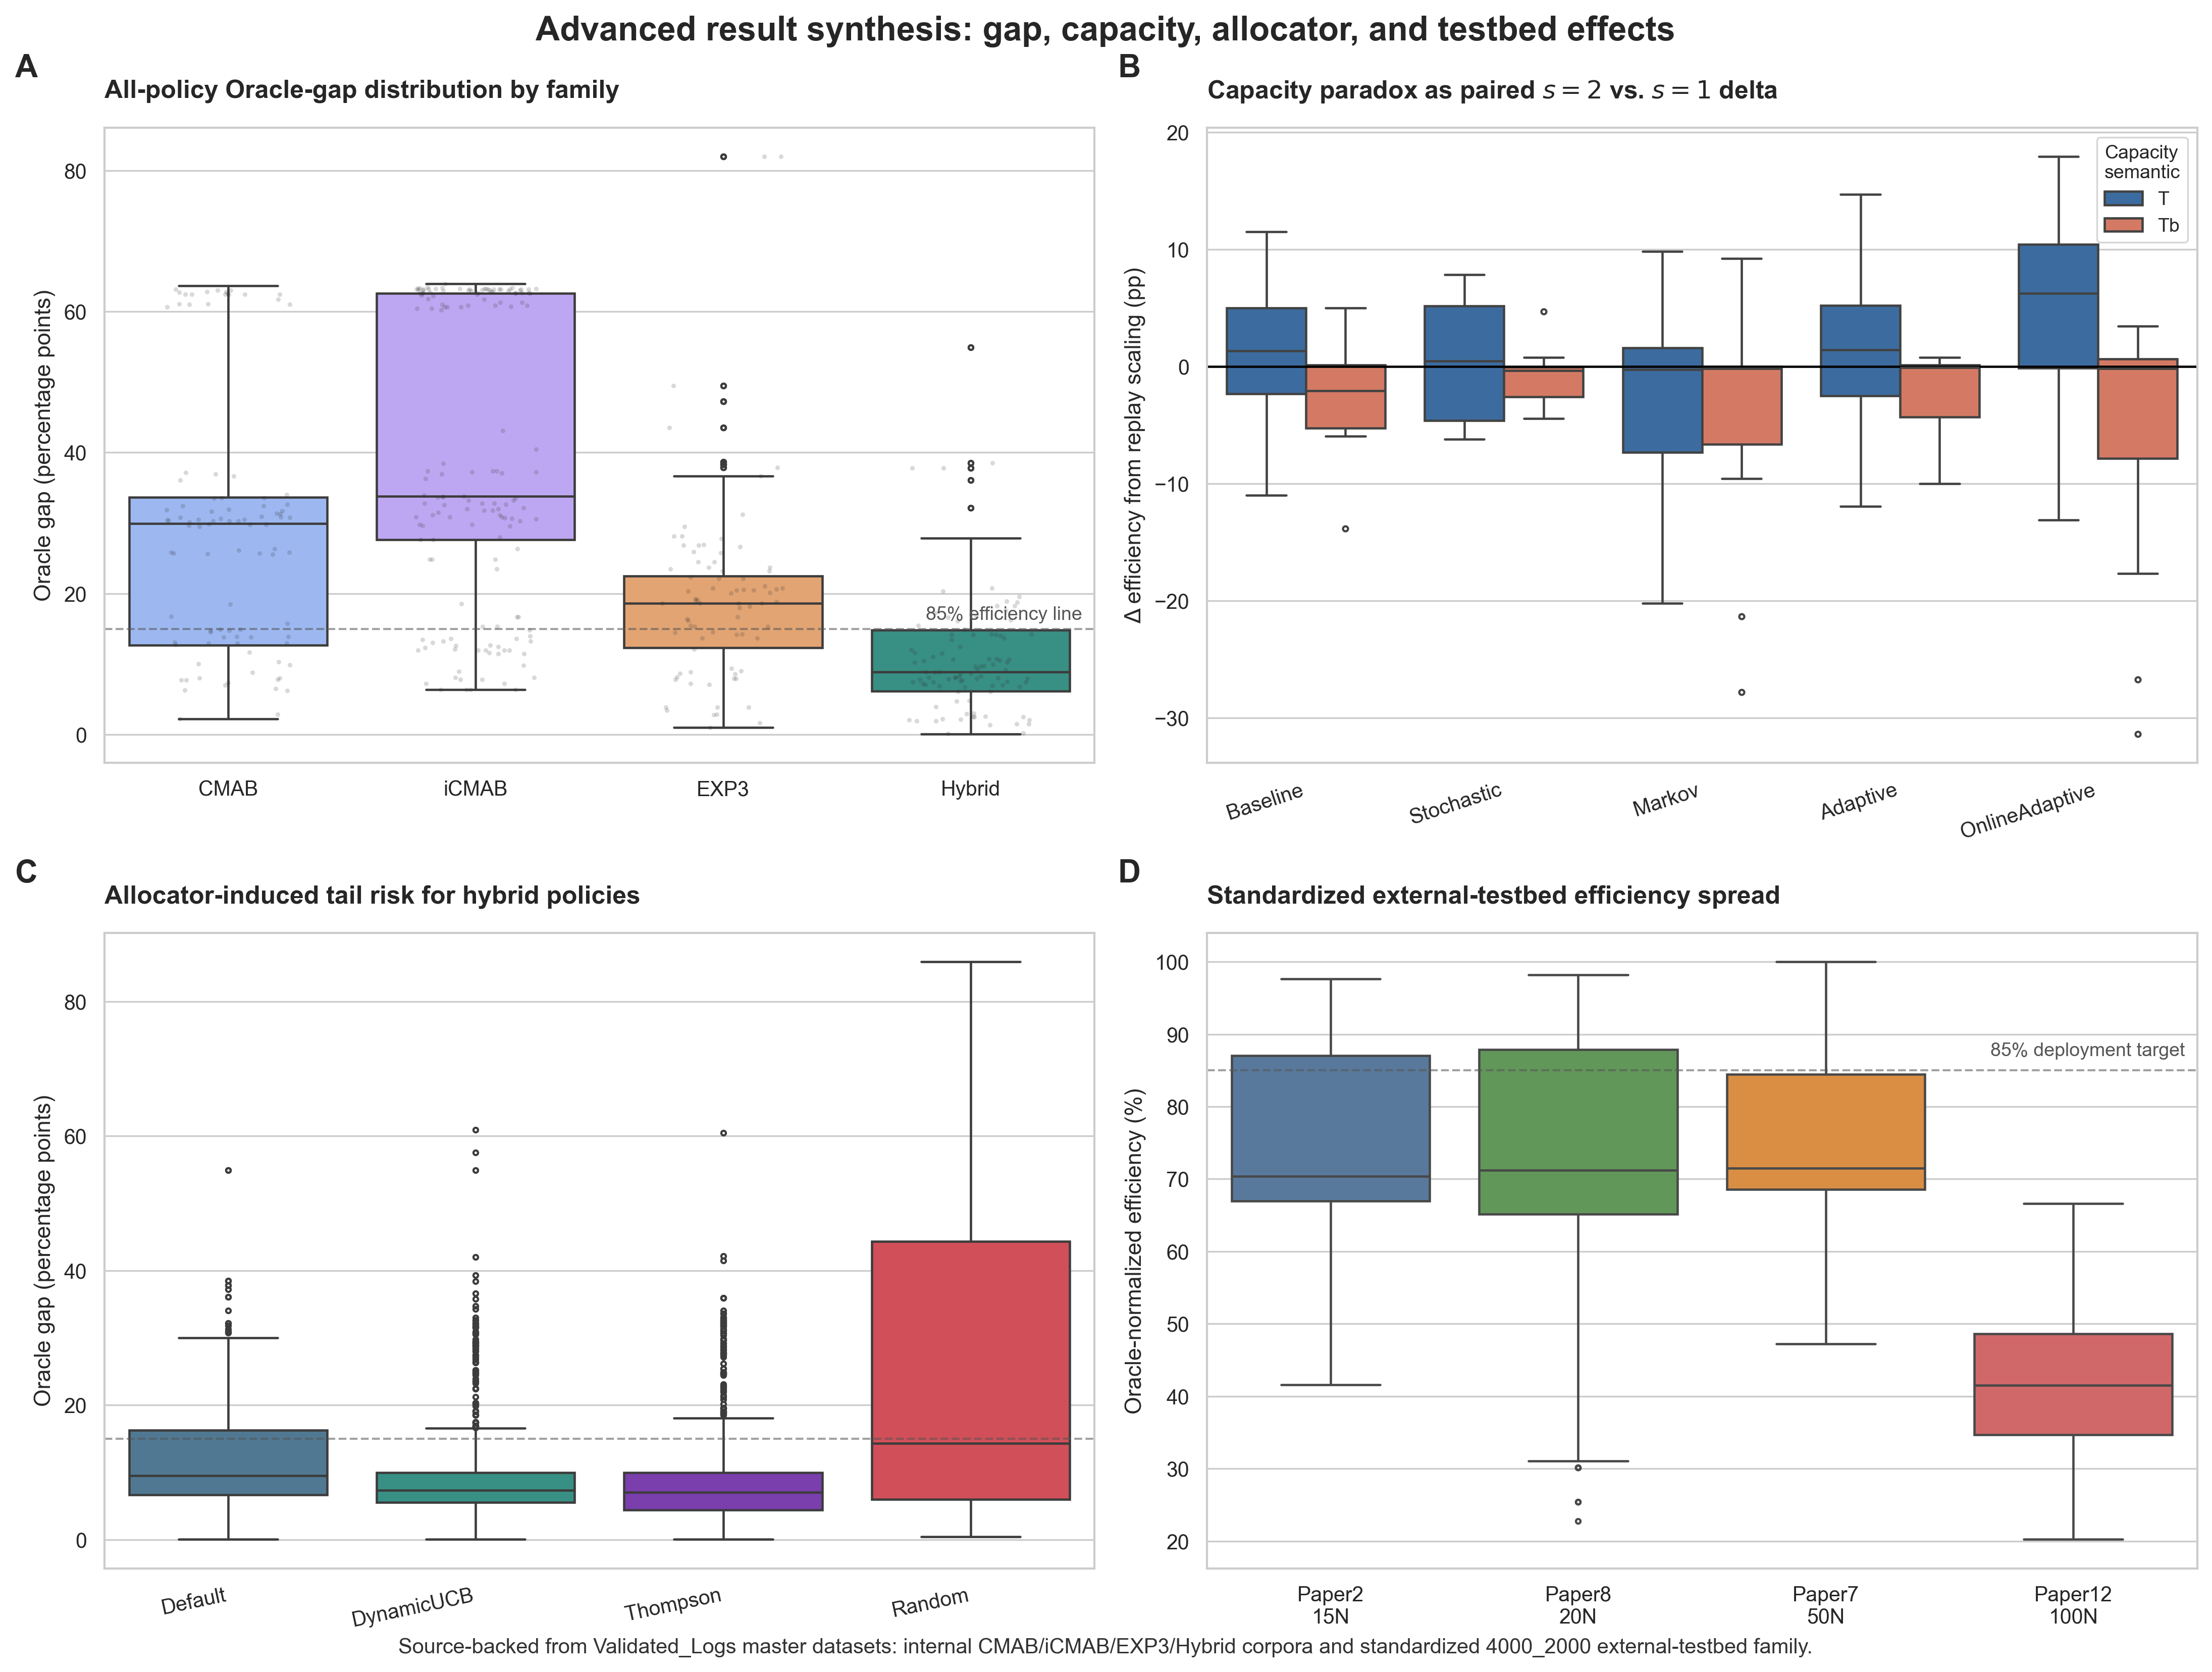
\includegraphics[width=\textwidth]{G7_advanced_synthesis.png}
    \caption{A four-panel synthesis links the paper's main claims: hybrid policies reduce Oracle gap, replay scaling has threat-dependent effects, allocator choice controls tail risk, and standardized testbeds expose topology-dependent efficiency spread.}
    \label{fig:plotpack_advanced_synthesis}
\end{figure*}

\begin{figure}[t]
    \centering
    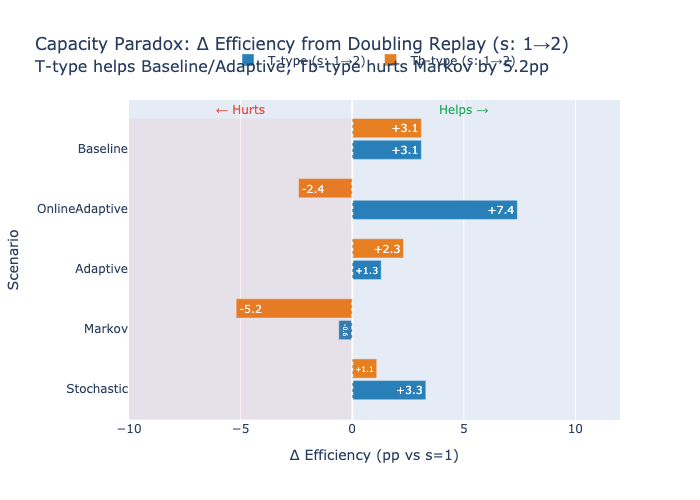
\includegraphics[width=\linewidth]{G1_capacity_paradox.png}
    \caption{Replay capacity has threat-dependent effects: doubling capacity helps several $T$ settings but hurts Markov under $T_b$, exposing the capacity paradox.}
    \label{fig:plotpack_capacity_paradox}
\end{figure}

\begin{figure}[t]
    \centering
    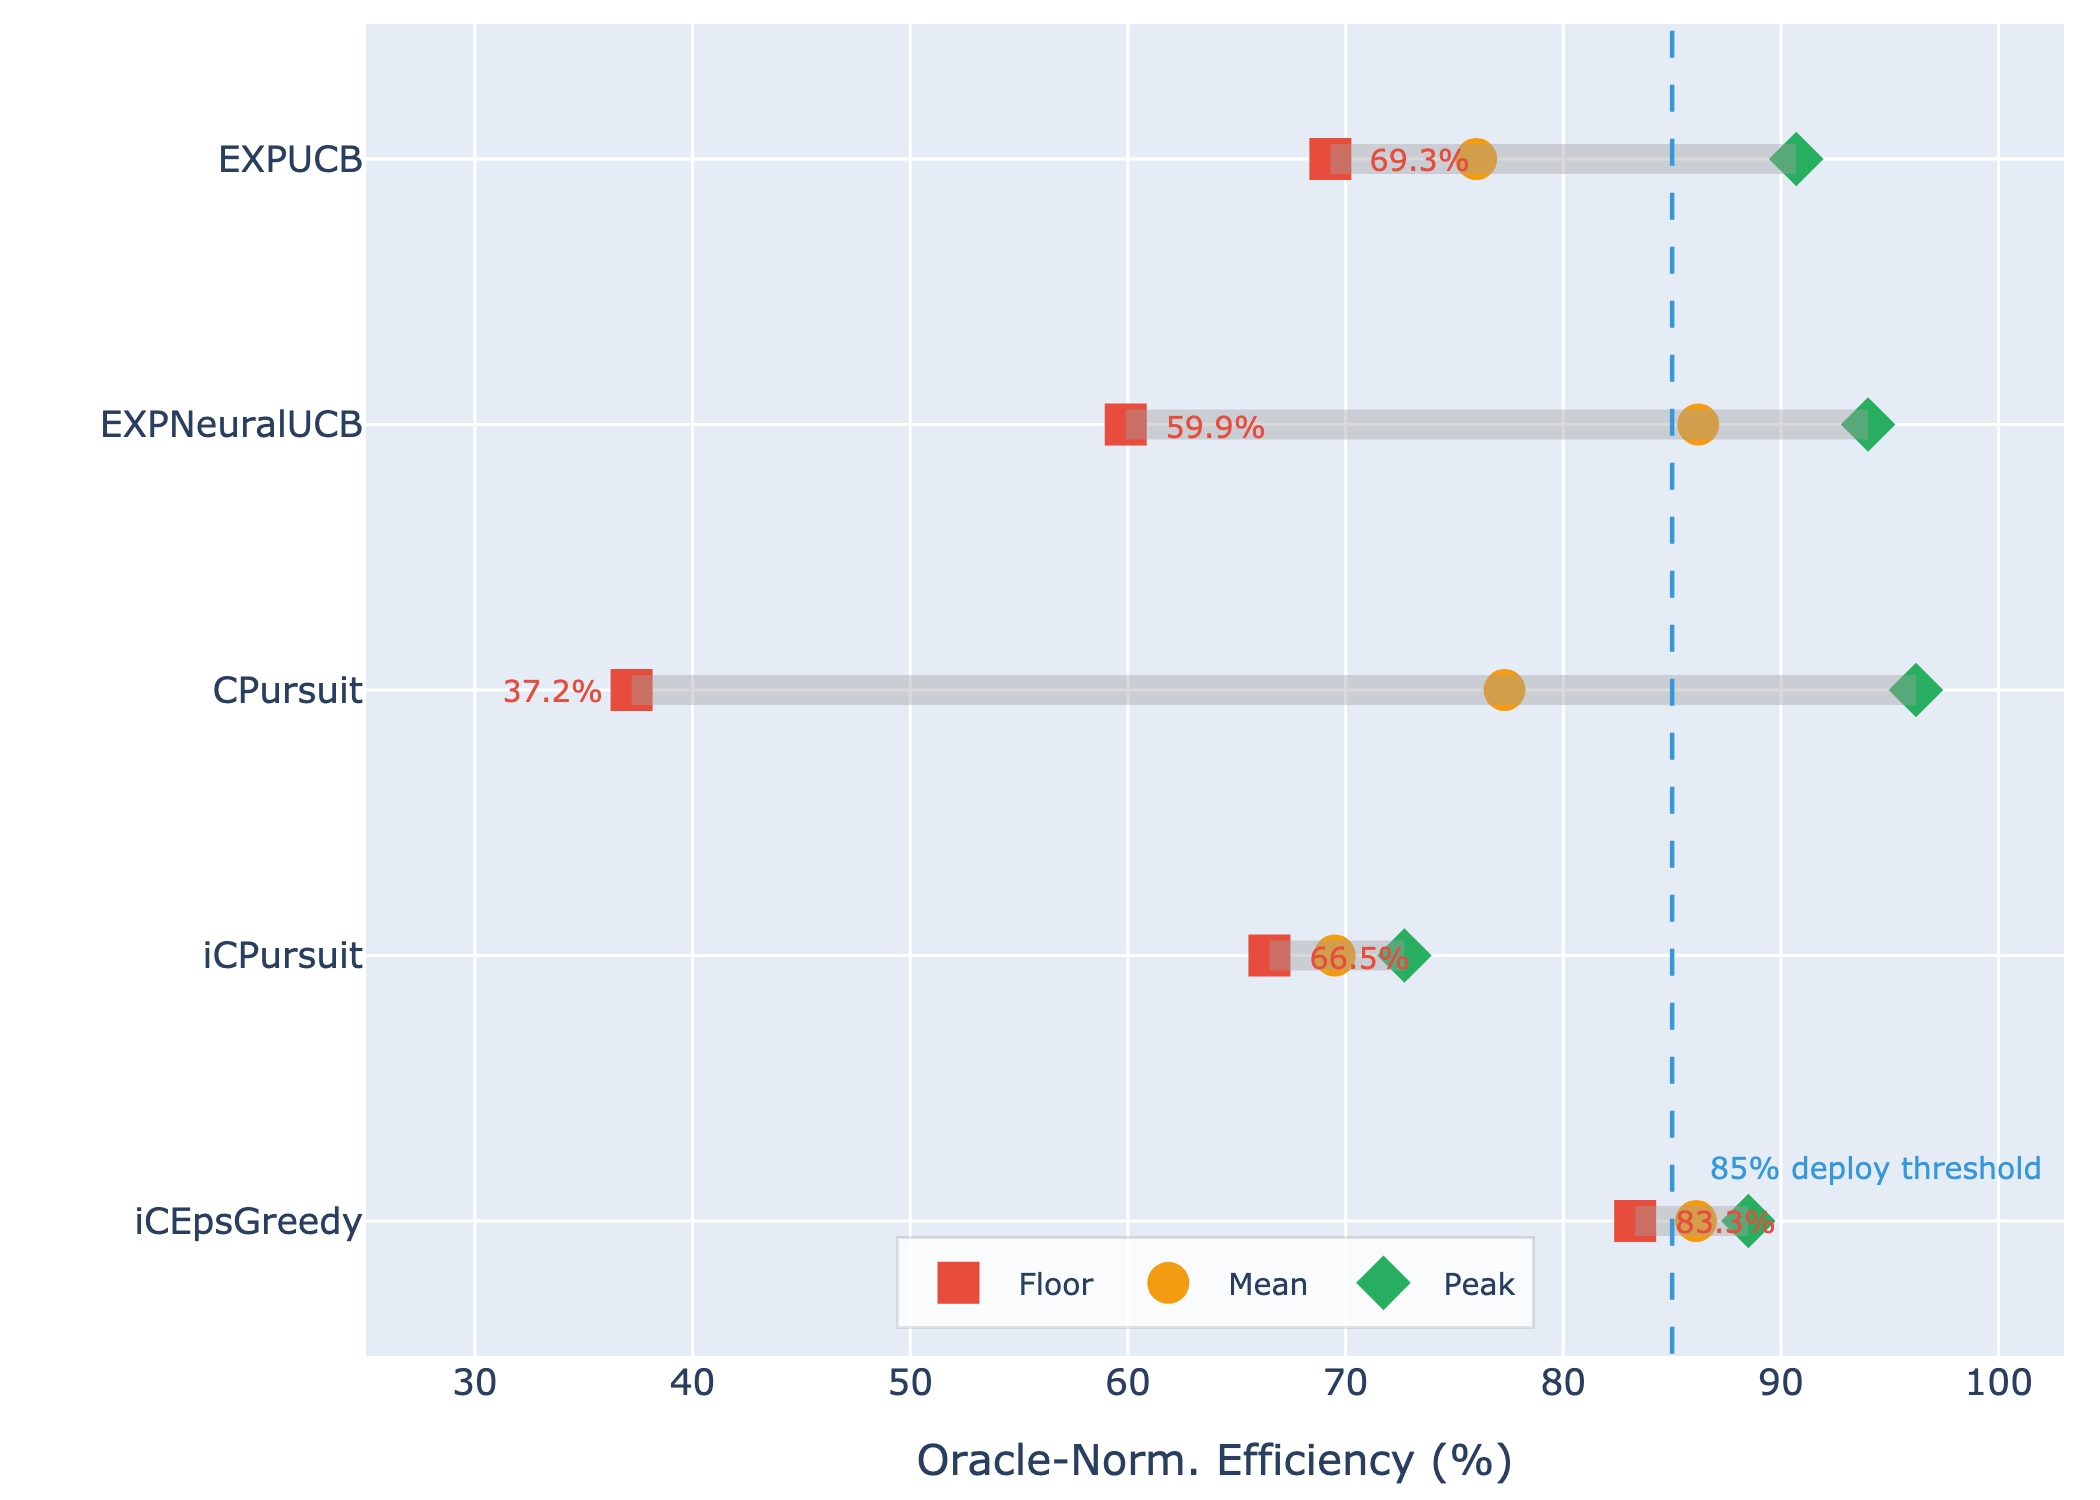
\includegraphics[width=\linewidth]{G2_robustness_floor.png}
    \caption{\texttt{iCEpsGreedy} maintains the strongest robustness floor, while \texttt{CPursuit} is most exposed under adaptive disruption.}
    \label{fig:plotpack_robustness_floor}
\end{figure}

\begin{figure}[t]
    \centering
    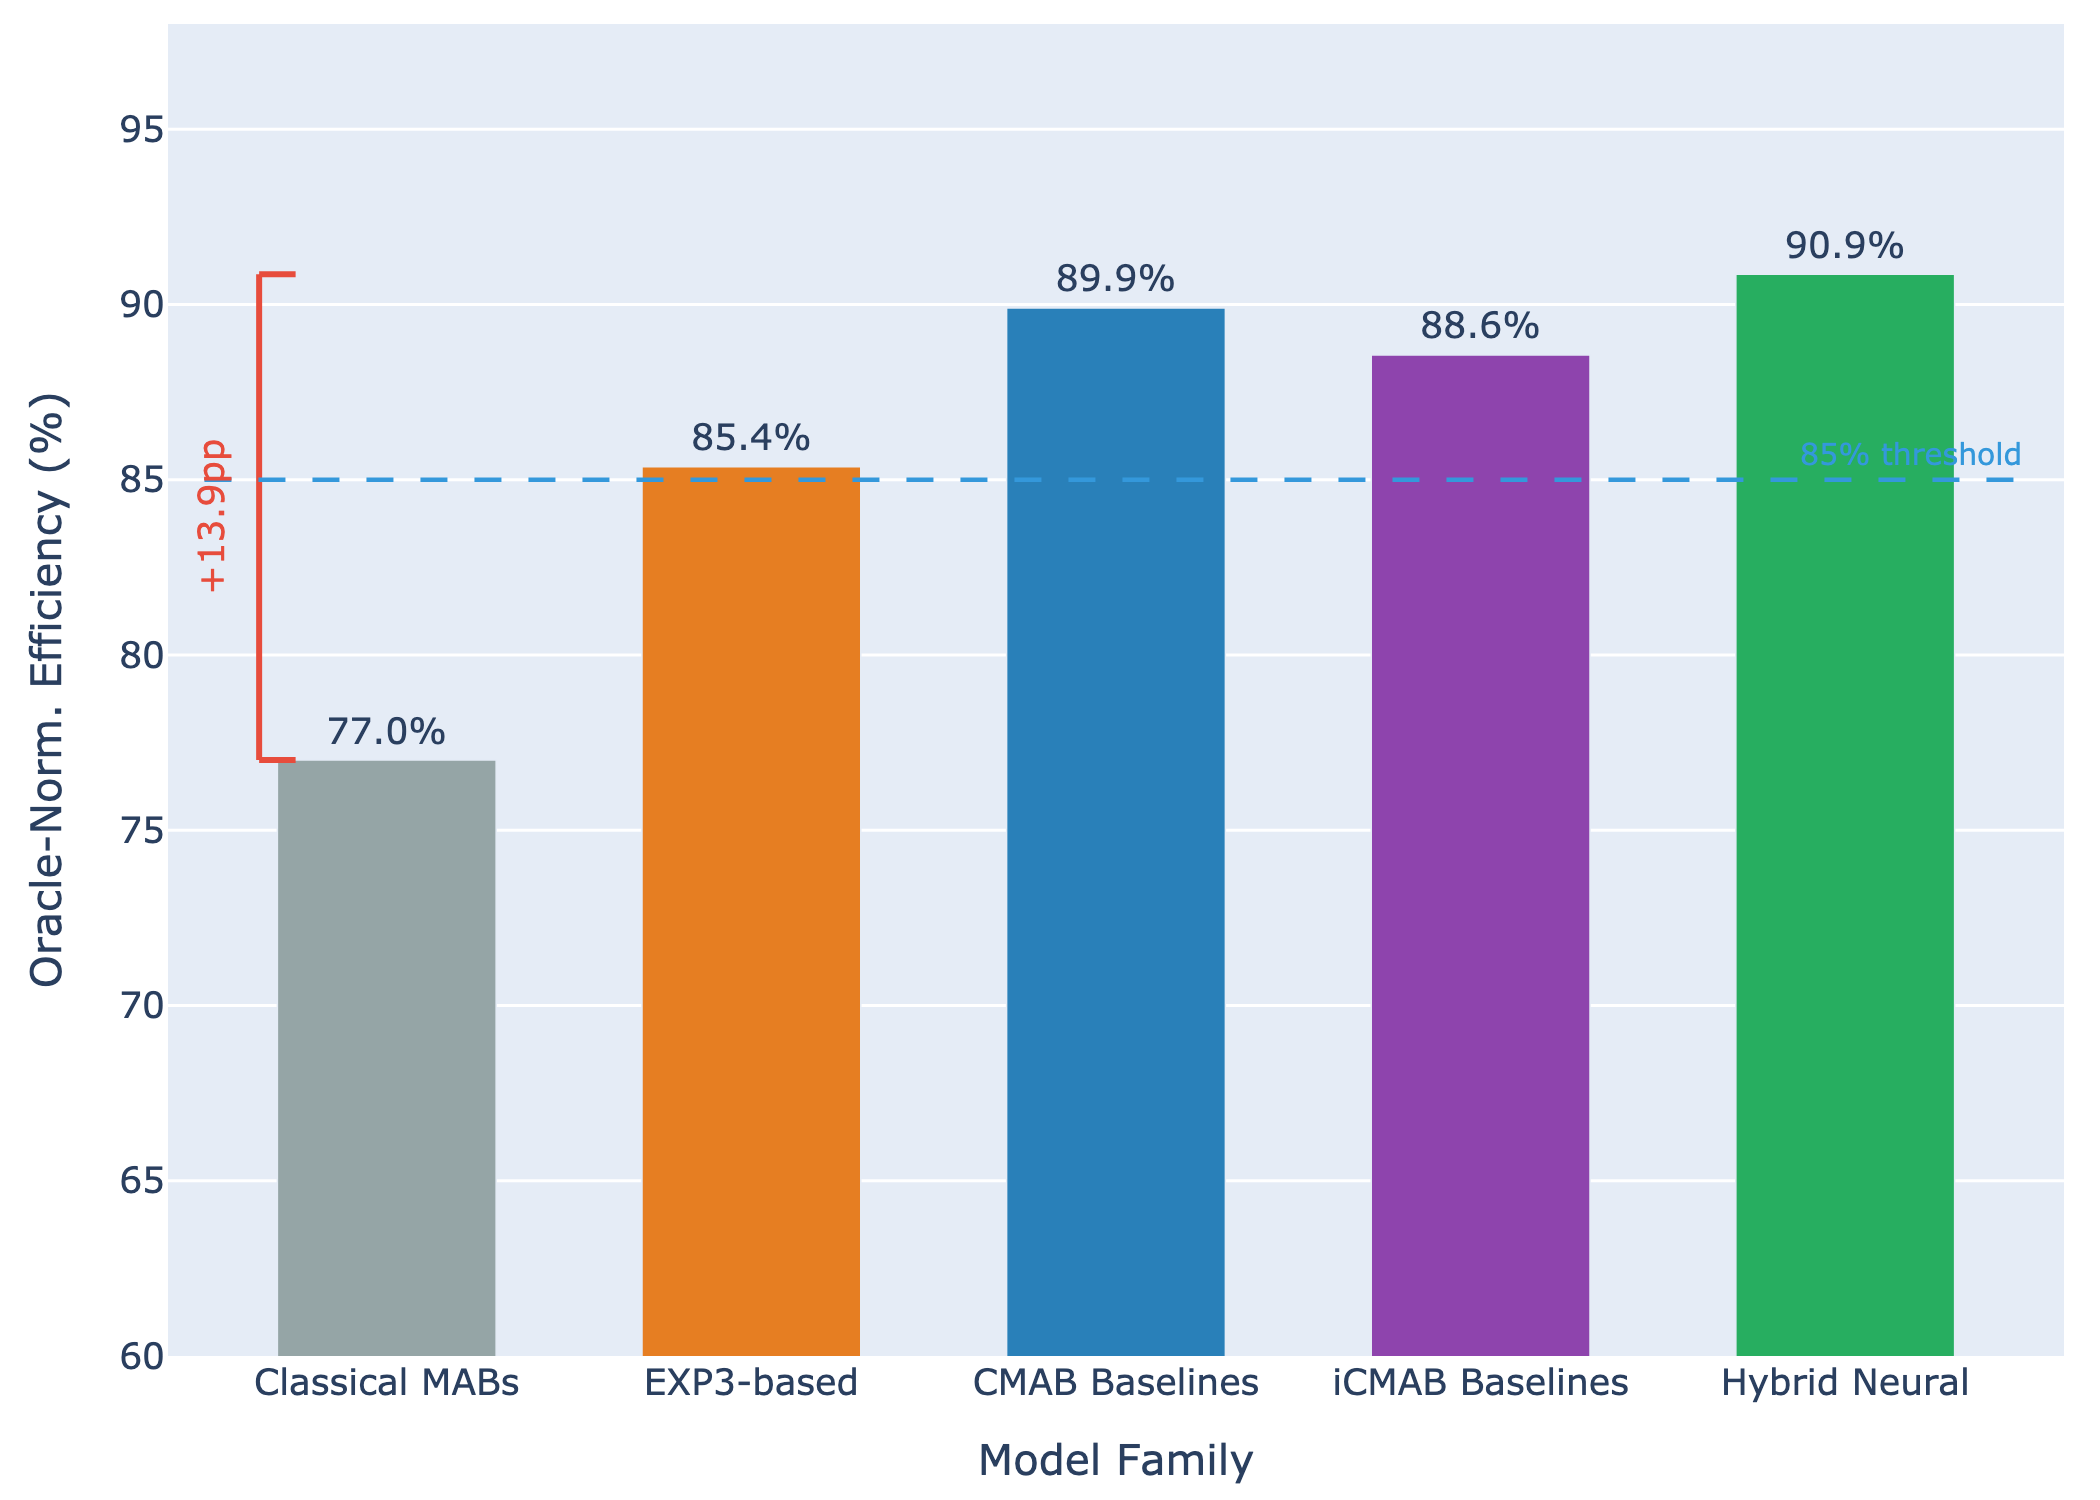
\includegraphics[width=\linewidth]{G3_family_summary.png}
    \caption{Hybrid neural and contextual families provide the strongest efficiency, with a clear gap over classical MAB baselines.}
    \label{fig:plotpack_family_summary}
\end{figure}

\begin{figure}[t]
    \centering
    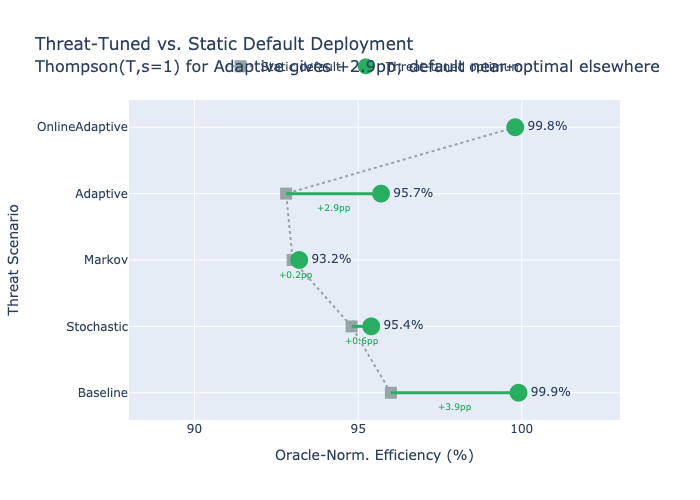
\includegraphics[width=\linewidth]{G4_deployment_rules.png}
    \caption{Threat-tuned deployment improves most in Adaptive and Baseline regimes, while the static default remains near-optimal elsewhere.}
    \label{fig:plotpack_deployment_rules}
\end{figure}

\begin{figure}[t]
    \centering
    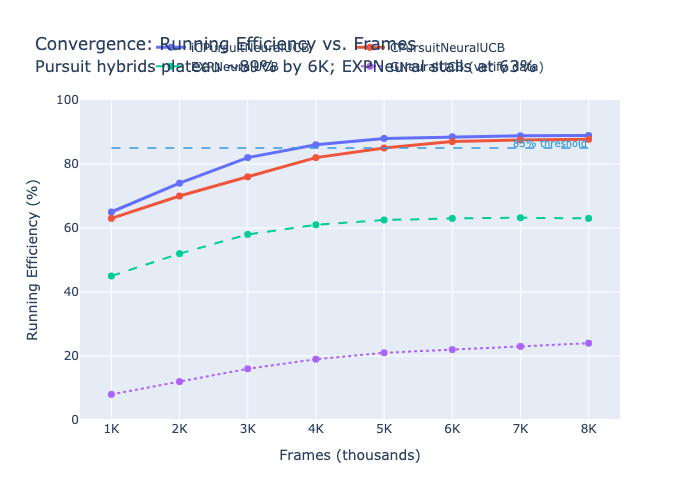
\includegraphics[width=\linewidth]{G5_convergence.png}
    \caption{Pursuit hybrids converge higher than neural and EXP3 baselines, but the \texttt{GNeuralUCB} curve remains a verification item before manuscript use.}
    \label{fig:plotpack_convergence}
\end{figure}

\begin{figure}[t]
    \centering
    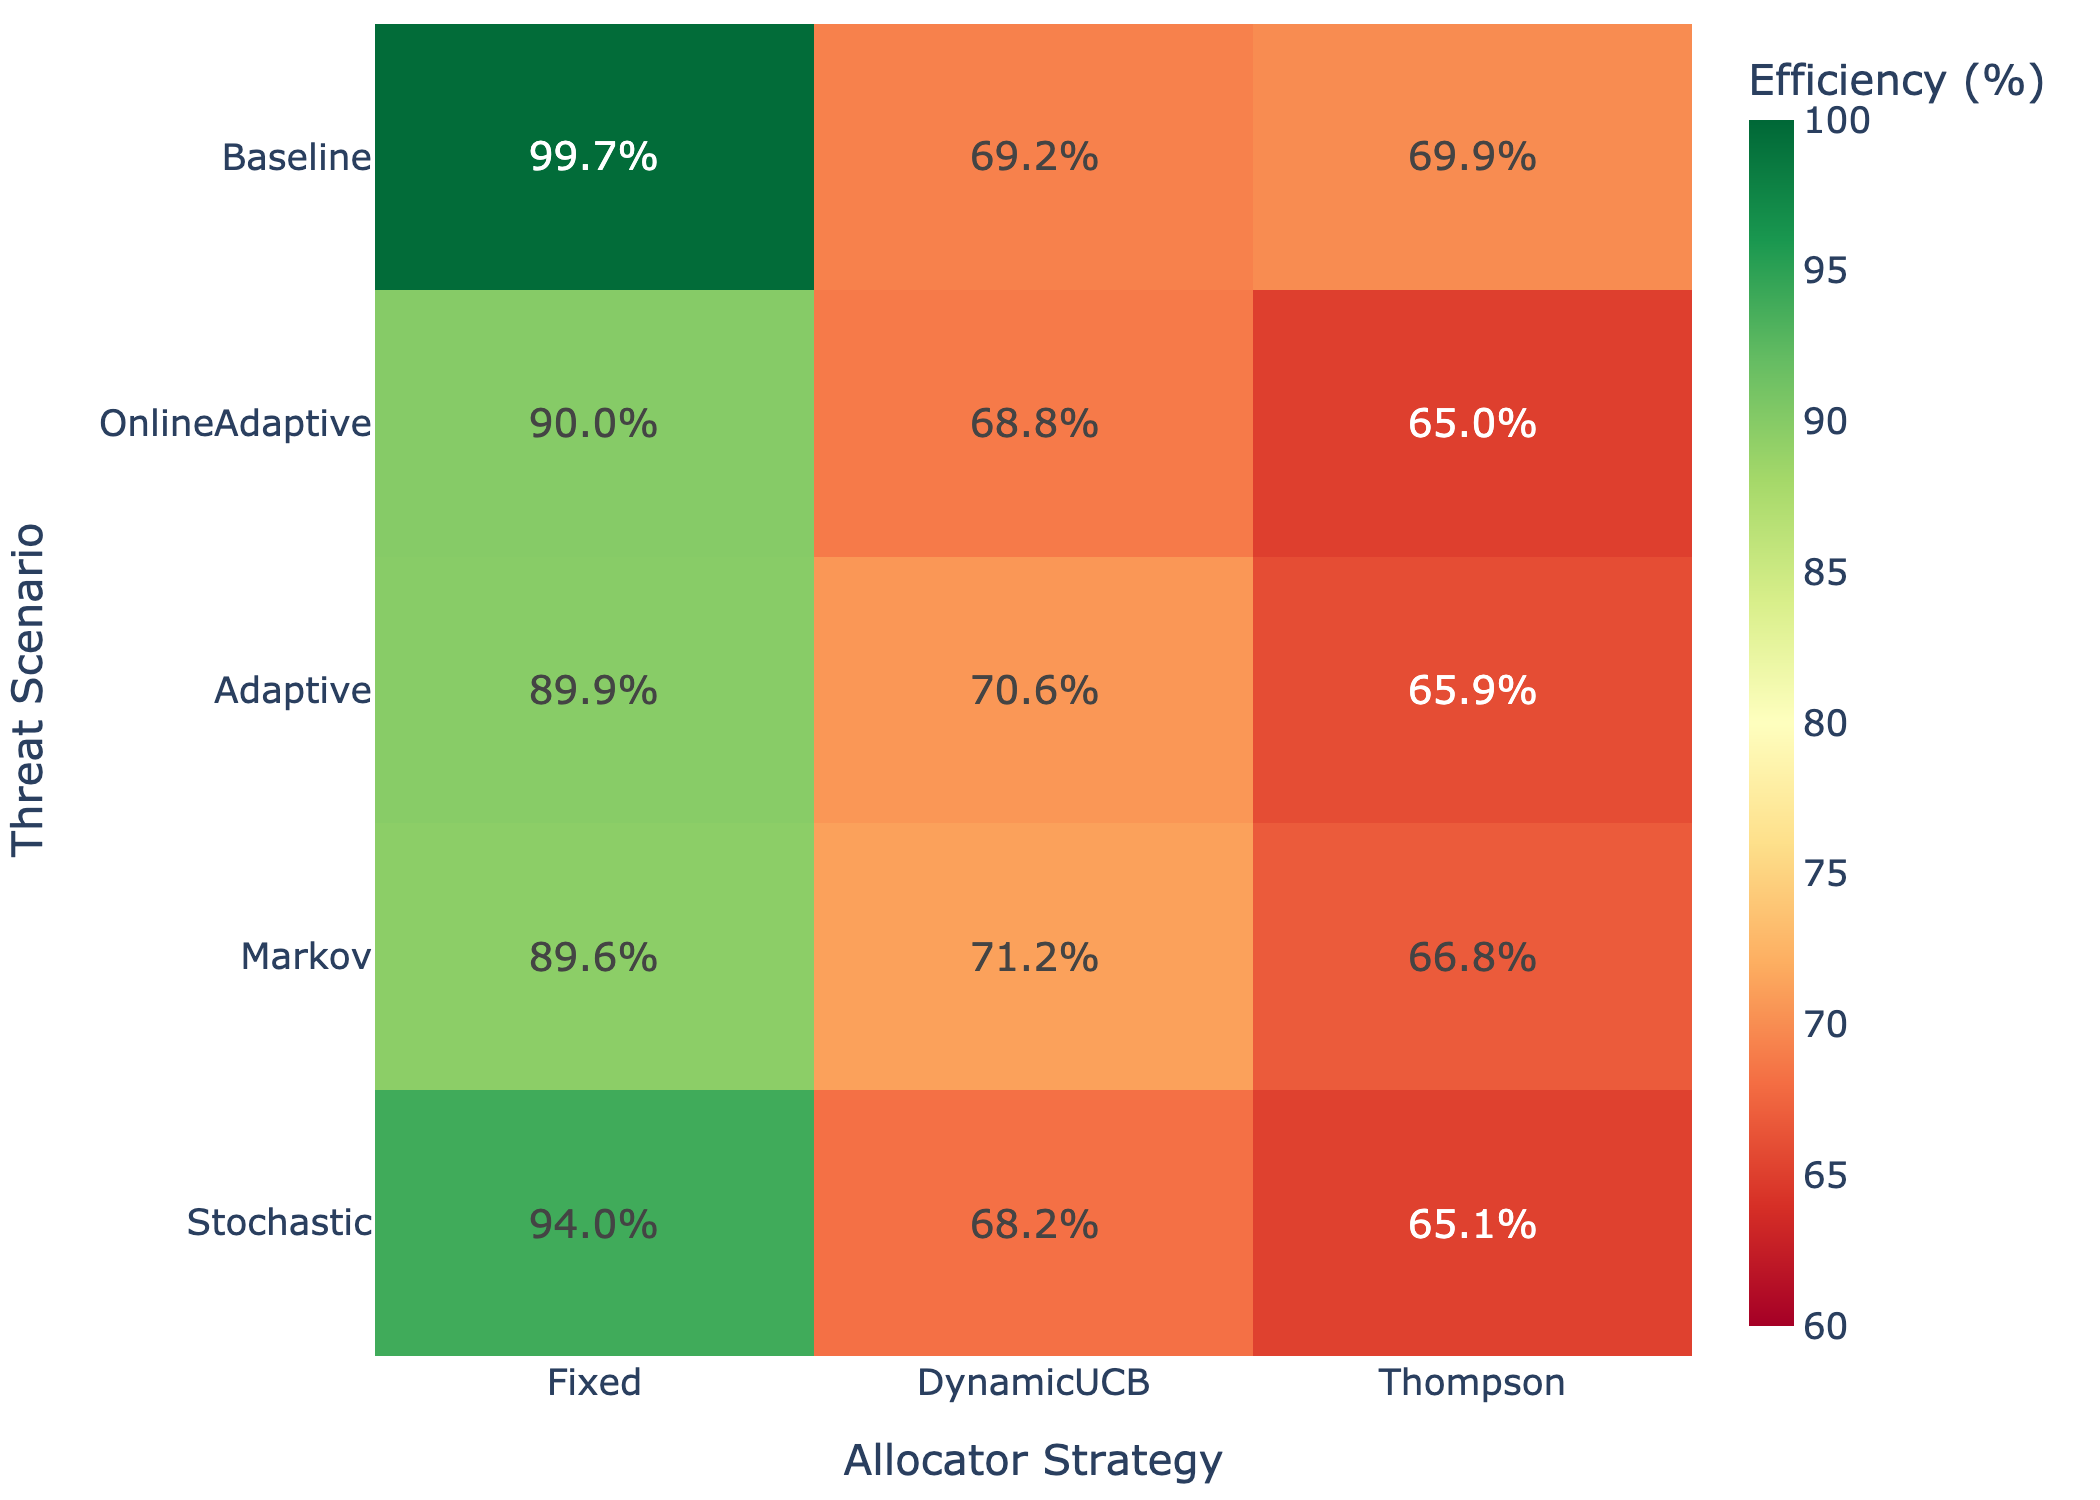
\includegraphics[width=\linewidth]{G6_heatmap.png}
    \caption{The Fixed allocator yields the highest \texttt{CPursuitNeuralUCB} efficiency across threat scenarios, reinforcing allocator choice as a robustness factor.}
    \label{fig:plotpack_heatmap}
\end{figure}

\section{Validation Notes}

The figures were generated from the local script under \texttt{tools/exported-assets-2/icnp\_graphs.py} using the \texttt{.quantum} environment. The local \texttt{tools/} directory is ignored by Git, so the tracked Overleaf-facing artifacts are the PNG files under \texttt{figures/icnp\_graphs/} and this standalone \texttt{.tex} file.

Figure~\ref{fig:plotpack_advanced_synthesis} is generated from the tracked G7 source script and summary CSV under \texttt{figures/icnp\_graphs/}; the inputs are the validated internal master datasets and the standardized \texttt{4000\_2000} external-testbed master dataset.

\textcolor{red}{Important:} Figure~\ref{fig:plotpack_convergence} keeps the original tool warning that the \texttt{GNeuralUCB} convergence series must be replaced with validated simulation output before it is used in the submission manuscript.

\end{document}
